\chapter{MUX time propagation delay }
In this chapter are presented the time delay calculations for all the previously showed multiplexers. Calculations have been performed using a "dividi et impera" approach, relying on the possibility to subdivide advanced multiplexer structures in  2-to-1 NAND2 based mux units. An RC delay model have been exploited, where the time constant of a single NAND gate is given by the total capacitance in the output node  times an effective resistance depending from the voltage source $V_{DD}$ and a ON current $I_{ON}$. In order to carry out quick estimations, we have considered a smart approach presented during lectures, referring on NAND2 statistical loads. Calculations have been done for CMOS MUX in HP, LOP and LSTP 2010 technologies.	

\section{Theoretical analysis}
According to the Roadmap, the average output of a NAND2 gate is fan-out of 4 made by inverters. It is therefore convenient to consider the total load capacitance of a NAND2 gate, as a sum of three different contributions
\begin{equation}
C_{ND2} = C_{FO4} + C_{metal} + C_J,
\end{equation}\\
where $C_{FO4}$ is an fan-out of 4 ideal statistical load, given by four inverters. The term $ C_{metal}$ accounts for capacitive contributions due to interconnects and $C_J$ accounts for junction capacitances. Overhead contributions of metallic interconnects and junctions have been estimated to be around 15\% of the ideal $C_{FO4}$.
It is possible to rewrite the previous expression in a more compact form
\begin{equation}
C_{ND2} = M \ C_{FO4},
\end{equation}
where $M$ has been fixed to  $1.5$ and plays the role of parasitic multiplier. According to theory,  $C_{FO4}$ is given by four times the value assumed by a simpler $C_{FO1}$ that can be written as $C_{FO1} = C_{gate_n}\ (1 + W_p/W_n) = 2.29 \  C_{gate_n}$. The nMOS gate capacitance can be expressed at first order by three different contributions involving the oxide capacitance, drain and source extension capacitances and a capacitance term modelling fringe effect. The capacitive contribution duo to the extensions has been considered 20\% of the oxide capacitance.  It is possible therefore to rewrite a plausible representation of the NAND2 load capacitance as a function of several CMOS technological parameters, taking into account all the three previously presented physical effects
\begin{equation}
C_{ND2} = 13.74 \left( \frac{\epsilon_{OX}}{t_{OX}} l_{ch} + 0.2 \frac{\epsilon_{OX}}{t_{OX}}  l_{ch} + C_{fringe}  \right) 
\end{equation}
Once the capacitances are known, it is necessary to evaluate the effective resistance. It can be represented as the ratio between the voltage source $V_{DD}$ and the ON current of a NAND2 gate ($I_{ND2_{ON}}$). In order to evaluate a worst-case situation, we consider the ON current of a NAND gate equal to the $I_{DS}$ current of a single pMOS transistor. This value has been evaluated using the Matlab MASTAR4 model reported in Tamtams. The effective resistance is given by the ratio $R = \frac{V_{DD}}{I_{ON}}$. The final value of the time constant of NAND2 gate is the simple RC product
\begin{equation}
\tau = R \ C_{ND2}.
\end{equation}

\subsection{MUX time delay}
The time delay evaluation in a multiplexer composed by a NAND tree structure follows simple rules.  In order to explain in a rigorous way the employed evaluation methodology, it is necessary to focus first the attention on a elementary block MUX 2x1. The critical path in a simple 2x1 mux is composed by three nand gates (see figure \ref{fig:mux2x1}) each one contributing for a unit of constant time. If we want to find the time delay of a 4x1 mux, it is necessary to consider a critical path defined by two 2x1 multiplexers connected in series. By extending this analysis to more advanced multiplexers, it is possible to write a generic expression for the total time delay, valid only in the simplified case of  multiplexers showing a nand tree structure
\begin{equation}
t = \tau \left[ 2 \log_2 (X) +1\right] 
\end{equation}
Where $X$ is the total number of input and is a power of two. Please notice that this general expression is unaffected by the parallelism $W$ of the system. In fact, increasing the parallelism will just affect the number of logic gates connected in parallel, without changing the critical path. Moreover, the simplicity of the expression is direct consequence of the choice to treat each nand gate in a statistical way, according to the roadmap recommendation.

\begin{figure}[!]
	\centering
	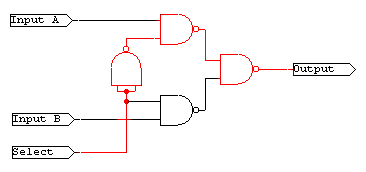
\includegraphics[scale =1]{capitoli/2x1}
	\caption{Representation of a 2x1 MUX. In red is highlighted the critical path.}
	\label{fig:mux2x1}
\end{figure}

\section{Simulation results}
Here are reported the time propagation delay numerical results of several multiplexers built according to the technologies HP, LSTP, LOP 2010. The simulations have been done for an arbitrary channel width $W_n = 270nm$. \\\\

\begin{tabular}{cccc}
	
	\cline{1-4}
	Number input    & HP & LOP & LSTP\\
	\hline
	2      & 35.58 ps    & 59.95 ps  &  59.96 ps  \\
	8  	  & 83 ps      & 130.6 ps    & 177.2ps  \\
	16       & 106.73 ps     & 167.9 ps    & 227.87 ps \\
	32       & 130.44 ps    & 205.15 ps     & 278.5 ps \\
	64 & 154.16 ps      & 242.44 ps      & 329.14 ps\\
	128 & 177.88 ps      & 279.74 ps     & 379.78 ps\\
	\hline
\end{tabular}
\\ \\
\subsection{Discussion}
In figure \ref{fig:time} are reported the simulation values together in a unique dispersion plot. As expected, the time delay of a high performance multiplexer shows smallest value with respect the other technologies. LSTP multiplexers are the slowest devices.
\begin{figure}[!]
	\centering
	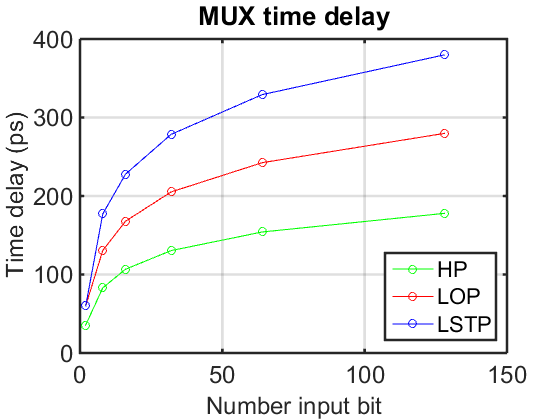
\includegraphics[scale =1]{capitoli/time}
	\caption{Time delay simulation results for 8, 16, 24, 32, 64, 128 inputs. Lines connecting each dot are just a graphical support.}
	\label{fig:time}
\end{figure}
\newpage

\section{Matlab implementation}
In the table below are reported the input data of the main script.

\begin{table}[h]
	\begin{center}
		\begin{tabular}{|c|c|c|c|} \hline
			\textbf{Quantity name} & \textbf{Description} & \textbf{u.m. (S.I.)} & \textbf{Variable name} \\ \hline
			$X$ &Number of input of MUX(is a power of 2) & / & X \\ 
			$C_{fringe}\ HP$ &Fringe capacitance MOS HP & F/nm & fring\_capHP2010 \\ 
			$C_{fringe} \ LOP$ &Fringe capacitance MOS LOP & F/nm & fring\_capLOP2010 \\ 
			$C_{fringe}\ LSTP$ &Fringe capacitance MOS LSTP & F/nm & fring\_capLSTP2010 \\
			$T_{ox}\ HP2010$ &Oxide thickness MOS HP2010 & nm & Tox\_HP2010 \\ 
			$T_{ox}\ LOP2010$ &Oxide thickness MOS LOP2010 & nm & Tox\_LOP2010 \\ 
			$T_{ox}\ LSTP2010$ &Oxide thickness MOS LSTP2010 & nm & Tox\_LSTP2010 \\
			$l_{ch}\ HP2010$ &channel length MOS HP2010 & nm & L\_HP2010 \\   
			$l_{ch}\ LOP2010$ &channel length MOS LOP2010 & nm & L\_LOP2010 \\
			$l_{ch}\ LSTP2010$ &channel length & nm & L\_LSTP2010 \\     
			$V_{DD}\ HP$ &Voltage source HP technology & V & Vdd\_HP2010 \\   
			$V_{DD}\ LOP$ &Voltage source LOP technology & V & Vdd\_LOP2010 \\ 
			$V_{DD}\ LSTP$ &Voltage source LSTP technology & V & Vdd\_LSTP2010 \\  \hline
		\end{tabular}
	\end{center}
	\caption{Input data}
	\label{tab1}
\end{table}

In the table below are reported the output data of the main script.

\begin{table}[h]
	\begin{center}
		\begin{tabular}{|c|c|c|c|} \hline
			\textbf{Quantity name} & \textbf{Description} & \textbf{u.m. (S.I.)} & \textbf{Variable name} \\ \hline
			$\tau \ HP2010$ &Time constant NAND2 HP2010 & s & Tsp\_HP\_nd2 \\
			$\tau \ LOP2010$ &Time constant NAND2 LOP2010 & s & Tsp\_LOP\_nd2 \\
			$\tau \ LSTP2010$ &Time constant NAND2 LSTP2010 & s & Tsp\_LSTP\_nd2 \\ 
			$t \ HP2010$ &Time delay mux HP2010 & s & tautotalHP \\
			$t \ LOP2010$ &Time delay mux LOP2010 & s & tautotalLOP \\
			$t \ LSTP2010$ &Time delay mux LSTP2010 & s & tautotalLSTP \\ \hline
		\end{tabular}
	\end{center}
	\caption{Output data}
	\label{tab1}
\end{table}
\subsection{Main time delay}
\begin{lstlisting}
%%%%%%%%%%%%%%%%%%%%%%%%%%%%%%%%%%%%%%%%%%%%%%%%%%%%
%                 MAIN Nand2 time delay                      
%%%%%%%%%%%%%%%%%%%%%%%%%%%%%%%%%%%%%%%%%%%%%%%%%%%%

clear all
close all

%Permittivity
eps_0 = 8.854187e-12 *1e-9; %F/nm
eps_SiO2 = 3.9*eps_0; %F/nm

%Fringe capacitances
fring_capHP2010 = 1.5e-16*1e-3; %F/nm
fring_capLOP2010 = 2.2e-16*1e-3;
fring_capLSTP2010 = 2.4e-16*1e-3;

%Oxide thickness
Tox_HP2010 = 0.65; %nm
Tox_LOP2010 = 0.9;
Tox_LSTP2010 = 1.4;

%Channel length
L_HP2010 = 18; %nm
L_LOP2010 = 22;
L_LSTP2010 = 28;

%Voltage source
VDD_HP2010 = 1; %V
VDD_LOP2010 = 0.7;
VDD_LSTP2010 = 1.1;

prompt = 'Specify the nMOS channel width Wn (nm):  ';
Wn = input(prompt)

%Total capacitance on output node of the Nand2 gate
C_nd2_HP = 13.74*(eps_SiO2*L_HP2010/Tox_HP2010 + fring_capHP2010 + ...
 0.2*eps_SiO2*L_HP2010/Tox_HP2010)*Wn;
C_nd2_LOP = 13.74*(eps_SiO2*L_LOP2010/Tox_LOP2010+fring_capLOP2010+ ...
0.2*eps_SiO2*L_LOP2010/Tox_LOP2010)*Wn;
C_nd2_LSTP=13.74*(eps_SiO2*L_LSTP2010/Tox_LSTP2010+fring_capLSTP2010 + ...
0.2*eps_SiO2*L_LSTP2010/Tox_LSTP2010)*Wn;

%Mastar model implementation
[Vth_nHP,Vth_pHP, Ioff_nHP, Ioff_pHP, Igate_nHP,...
Igate_pHP]= Mastar4_Vth_Ioff_IgHP2010();
[I_nMOSHP, I_pMOSHP]= Ion_Mastar_modelHP2010(Vth_nHP); %uA/um

[Vth_nLOP,Vth_pLOP, Ioff_nLOP, Ioff_pLOP, ...
Igate_nLOP, Igate_pLOP]= Mastar4_Vth_Ioff_IgLOP2010();
[I_nMOSLOP, I_pMOSLOP]= Ion_Mastar_modelLOP2010(Vth_nLOP); %uA/um

[Vth_nLSTP,Vth_pLSTP, Ioff_nLSTP, Ioff_pLSTP, ...
Igate_nLSTP, Igate_pLSTP]= Mastar4_Vth_Ioff_IgLSTP2010();
[I_nMOSLSTP, I_pMOSLSTP]= Ion_Mastar_modelLSTP2010(Vth_nLSTP); %uA/um

%NAND2 delay evaluation
Wp = 1.29*Wn;
Tdp_HP_nd2 =C_nd2_HP*VDD_HP2010/(I_pMOSHP*Wp*1e-3*1e-6); %s
Tdp_LOP_nd2 =C_nd2_LOP*VDD_LOP2010/(I_pMOSLOP*Wp*1e-3*1e-6); %s
Tdp_LSTP_nd2 =C_nd2_LSTP*VDD_LSTP2010/(I_pMOSLSTP*Wp*1e-3*1e-6); %s

prompt = 'Specify the number of channel inputs:  ';

X = input(prompt);
%Ninput has a mean only if is 2,4,8,16,32,64

%Time delay evaluation, s
tautotalHP =log2(X)*2*Tdp_HP_nd2+Tdp_HP_nd2 %s
tautotalLOP =log2(X)*2*Tdp_LOP_nd2+Tdp_LOP_nd2 %s
tautotalLSTP =log2(X)*2*Tdp_LSTP_nd2+Tdp_LSTP_nd2 %s
\end{lstlisting}

\subsection{Mastar4 Vth Ioff Ig HP2010()}
This is a function needed in order to evaluate the threshold voltages, the off and the gate current of MOS transistors.
The most part of the code has been taken from the Matlab modules of TAMTAMS.

\begin{lstlisting}
function [Vth_n,Vth_p, Ioff_n, Ioff_p, Igate_n,...
Igate_p]= Mastar4_Vth_Ioff_IgHP2010()
%Please see: https://tamtams.vlsilab.polito.it/...
%Documentation/TechnologyHTML/bulk/HP2010_dev_bul.html

%PARAMETERS           
%Please, select "Model" value for the technology type
%BULK = 0; FINFET = 1; SOI = 2; GAA = 3; CNT = 4;
Model = 0; 

%Physical parameters
q = 1.6021766208e-19;     % elementary charge (C)
kB = 1.3806488e-23;       % Boltzmann constant (J/K)
hbar = 1.054571800e-34;   % reduced Planck cons tant (Js)
m0 = 9.10938291e-31;      % electron mass (kg)
clight = 2.99792458e8 ;   % speed of light (m/s)
mu0 = (4* pi )*1e-7;      % vacuum magnetic permeability (H/m)
e0 = 1e-2/( clight ^2* mu0 );% vacuum electric permittivity (F/cm)
es = 11.8;                % Silicon relative dielectric constant
esio2 = 3.9;              % Silicon oxide relative dielectric constant
Eg0 = 1.166;              % Silicon energy gap at 300K (eV)
Alpha = 4.73e-4; Beta = 636;
Temp = 300;               % Absolute working temperature (K)
Eg = Eg0 - Alpha * Temp^2/(Temp + Beta);%Silicon energy gap (eV)
Vt = kB.*Temp./q;         %Termal voltage (V)
ni = sqrt(5.85e31*Temp^3*exp(-Eg/Vt));%Intrinsic carrier concentration(cm^-3)
Xs = 4.003;               % Silicon affinity (eV)

%Geometrical parameters (HP 2012)
Lgate =18; %nm, The effective length of the gate.
Xj = 6.5; %nm, Source/Drain extensions length.
LDDW = 50; %nm, Doping width of source/drain extension, value used only...
%for transistors image generation.
Tox = 0.65; %nm, Physical gate oxide thickness.
Darks = 0.27; %nm, 2.5 A=0.1nm Dark space length, used in...
%Mastar threshold voltage model.
Polyd = 0; %Poly depletion length, used in Mastar threshold voltage model.
Wt = 1000; %nm, Gate width of n-MOS.
beta =1.29; %is the ratio between Wp/Wn.
gateW_p = beta*Wt; %nm, Gate width of p-MOS
gateH = 40; %nm, Gate thickness, 
DopH = 30; %nm, Doping depth of source/drain
DopW = 100; %nm, Doping width of source/drain
ContW = 30; %nm, Contact width
Diff_ray = 5;%nm, Ray of annealing diffusion
Angle = 25; %deg, Pocket implantation angle

%Doping parameters (HP 2010)
Nbulk = 7.14e18; %cm^-3, Channel Doping
n_sub = 3.2e18; %cm^-3, Substrate Doping
n_plus_poly = 1e20; %cm^-3, Polysilicon n+ doping
Next = 7.819e18; %cm^-3, Extensions doping
n_source_drain = 1e20; %cm^-3, Source/Drain doping

%Electrical parameters (HP 2010)
rconst_n = 254.61; %Ohm, N-MOS access resistance
rconst_p = 254.61; %Ohm, P-MOS access resistance
Fring_cap = 1.5e-16; %F/um, Fringe capacitance per unit length
Ith = 5e-7; %A, Id at the threshold voltage (Vth_off)
Phi_m = 4.15; %V Built-in potential
Kfield = 1; %Effective electric field reduction

%Scaling factors (HP 2010)
Gamma = 0.7; % Scaling factor for lateral diffusion
Zeta = 0.8; %Scaling factor for drain induced lowering barrier (DIBL)
Zeta2 = 0.64; %Scaling factor for short channel effect (SCE)

%Power supply parameters (HP 2010)
Vdd = 1; %V Operation voltage (gate and drain voltages)

%Other parameters(HP 2010)
Cpoches = 5.2e13;
Rp = 10; %nm
Delta_rp = 6; %nm
Delta_rl = 3; %nm
ActivePkt = 0;


%THRESHOLD VOLTAGE, MASTAR 4 MODEL
% https://tamtams.vlsilab.polito.it/Documentation/ ...
ModulesHTML/vth/vth_mas_complete_bul.html

ni_temp = ni /3.79; %Fitting from Mastar
Phi_f = Vt*log(Nbulk/ni_temp); %Surface potential (V)
Vfb= Phi_m -(Xs + Eg/2 + Phi_f);
Vbi=Vt*log(Nbulk*Next/ni_temp^2);
Qdep=sqrt(2*es*e0*q*Nbulk*(2*Phi_f));
Tox_el=Tox*3.9/esio2 + Darks/10 + Polyd/10; %nm, Electrical oxide thickness 
% %considering the effect of Dark Space and Polysilicon depletion
Cox=esio2*e0/(Tox_el*1e-7); %Oxide capacitance evaluation [F/cm^2]
Vtlong=Vfb+2*Phi_f+Qdep/Cox; %Long channel threshold voltage
Lel=Lgate-Gamma*Xj; %Channel electric length [nm]

%Depletion depth calculation:
Tdepbulk=1e7*Qdep/(q*Nbulk);
% for BULK transistors
if(Model==0)
Tdep=Tdepbulk;
% for Double Gate transistors
elseif(Model==1)
Tdep=Xj/2;
Xj=Xj/2;
% for SOI transistors
else if (Tdepbulk<Xj)
Tdep=Tdepbulk;
else
Tdep=Xj;
end
end

EI=(1+(Xj/Lel)^2)*Tox_el*Tdep/(Lel)^2;
% Short Channel Effect (SCE) [V]
SCE=es/esio2*Zeta2*Vbi*EI;
% Drain Induced Barrier Lowering (DIBL) [V]
DIBL=es/esio2*Zeta*EI*Vdd;
Vth=Vtlong-SCE-DIBL;
Vth_n = Vth;
Vth_p = -Vth;


%SUBTHRESHOLD CURRENT, MASTAR 4 MODEL
% https://tamtams.vlsilab.polito.it/Documentation/...
ModulesHTML/ioff/Ioff_mas4_bul.html


Npocket=0.5*(Cpoches/((Rp+2*Delta_rp)*10^-7)); 
Lpocket=(Rp+2*Delta_rp)*sin(Angle*pi/180)+ ...
2*Delta_rl*cos(Angle*pi/180)-(Gamma*Xj)/2;
Lel = Lgate - Gamma * Xj; %Electrical channel length [nm]
Lmin=min(Lel,Lpocket); %Effective channel length
Nch = Nbulk + 2 * Npocket * (Lmin/Lel); %Channel doping
if (ActivePkt==0)
Ith_new = Ith*Wt/Lel;
else
Ith_new = Ith*Wt/Lel* 8 * 10^8 * Nch^(-0.4865);
end;

Qdep = sqrt(2*es*e0*q*Nbulk*(2*Phi_f)); %Depletion charge evaluation

%Depletion depth calculation
Tdepbulk=1e7*Qdep/(q*Nbulk);
% for BULK transistors
if(Model==0)
Tdep=Tdepbulk;
% for Double Gate transistors
elseif(Model==1)
Tdep=Xj/2;
Xj=Xj/2;
% for SOI transistors
else if (Tdepbulk<Xj)
Tdep=Tdepbulk;
else
Tdep=Xj;
end
end

SS=Vt*log(10)*(1+((es/esio2)*Kfield*(Tox_el/Tdepbulk))); %V/dec
Ioff_n=Ith_new*10^(-Vth/SS)*10^9;  %nA/um
Ioff_p=Ith_new*10^(-Vth/SS)*10^9;  %nA/um


% GATE CURRENT, MASTAR 4 MODEL
% https://tamtams.vlsilab.polito.it/Documentation/...
ModulesHTML/igate/Igate_Mastar4_bul.html

%a, b, c, d parameters:
ag = 1.44e5;	% A/cm^2
bg = -4.02;		% V^-2
cg = 13.05;		% V^-1
dg = 1.17;		% Angstrom^-1

%Gate current density
Jgate_n = ag*exp(bg*Vdd^2 + cg*Vdd)*exp(-dg*Tox*10)*10;	% nA/um^2
Jgate_p = ag*exp(bg*Vdd^2 + cg*Vdd)*exp(-dg*Tox*10)*10;

Igate_n= Jgate_n*Lgate*1e-3; % [nA/um]
Igate_p= Jgate_p*Lgate*1e-3; % [nA/um]

if (Model==1)
Igate_n=2*Igate_n;
Igate_p=2*Igate_p;
end
return
\end{lstlisting}

The other two functions Mastar4\_Vth\_Ioff\_IgLOP2010() and Mastar4\_Vth\_Ioff\_IgLSTP2010() are not reported here, since they change just for what concern constants. For more details please see the original Matlab scripts.

\subsection{Ion Master model HP 2010()}
This is a function needed in order to evaluate the $I_{ON}$ of MOS transistors.
The most part of the code has been taken from the Matlab modules of TAMTAMS.

\begin{lstlisting}
function [Ion_n, Ion_p]= Ion_Mastar_modelHP2010(Vth)

% PARAMETERS                
%Please, select "Model" value for the technology type
%BULK = 0; FINFET = 1; SOI = 2; GAA = 3; CNT = 4;
Model = 0; 

%Physical parameters
q = 1.6021766208e-19;     % elementary charge (C)
kB = 1.3806488e-23;       % Boltzmann constant (J/K)
hbar = 1.054571800e-34;   % reduced Planck cons tant (Js)
m0 = 9.10938291e-31;      % electron mass (kg)
clight = 2.99792458e8 ;   % speed of light (m/s)
mu0 = (4* pi )*1e-7;      % vacuum magnetic permeability (H/m)
e0 = 1e-2/( clight ^2* mu0 ); % vacuum electric permittivity (F/cm)
es = 11.8;                % Silicon relative dielectric constant
esio2 = 3.9;              % Silicon oxide relative dielectric constant
Eg0 = 1.166;              % Silicon energy gap at 300K (eV)
Alpha = 4.73e-4; Beta = 636;
Temp = 300;                % Absolute working temperature (K)
Eg = Eg0 - Alpha * Temp^2/(Temp + Beta);%Silicon energy gap (eV)
Vt = kB.*Temp./q;          %Termal voltage (V)
ni = sqrt(5.85e31*Temp^3*exp(-Eg/Vt)); %Intrinsic carrier concentration(cm^-3)
Xs = 4.003;                % Silicon affinity (eV)

%Geometrical parameters (HP 2010)
Lgate =18; %nm, The effective length of the gate.
Xj = 6.5; %nm, Source/Drain extensions length.
LDDW = 50; %nm, Doping width of source/drain extension
Tox = 0.65; %nm, Physical gate oxide thickness.
Darks = 0.27; %nm, 2.5 A=0.1nm Dark space length
Polyd = 0; %Poly depletion length
Wt = 1000; %nm, Gate width of n-MOS.
beta =1.29; %is the ratio between Wp/Wn.
gateW_p = beta*Wt; %nm, Gate width of p-MOS
gateH = 40; %nm, Gate thickness
DopH = 30; %nm, Doping depth of source/drain
DopW = 100; %nm, Doping width of source/drain
ContW = 30; %nm, Contact width
Diff_ray = 5;%nm, Ray of annealing diffusion
Angle = 25; %deg, Pocket implantation angle

%Doping parameters (HP 2010)
Nbulk = 7.14e18; %cm^-3, Channel Doping
n_sub = 3.2e18; %cm^-3, Substrate Doping
n_plus_poly = 1e20; %cm^-3, Polysilicon n+ doping
Next = 7.819e18; %cm^-3, Extensions doping
n_source_drain = 1e20; %cm^-3, Source/Drain doping

%Electrical parameters (HP 2010)
rconst_n = 254.61; %Ohm, N-MOS access resistance
rconst_p = 254.61; %Ohm, P-MOS access resistance
Fring_cap = 1.5e-16; %F/um, Fringe capacitance per unit length
Ith = 5e-7; %A, Id at the threshold voltage (Vth_off)
Phi_m = 4.15; %V Built-in potential
Kfield = 1; %Effective electric field reduction

%Scaling factors (HP 2010)
Gamma = 0.7; % Scaling factor for lateral diffusion
Zeta = 0.8; %Scaling factor for drain induced lowering barrier (DIBL)
Zeta2 = 0.64; %Scaling factor for short channel effect (SCE)

%Power supply parameters (HP 2010)
Vdd = 1; %V Operation voltage (gate and drain voltages)

%Other parameters(HP 2010)
Cpoches = 5.2e13;
Rp = 10; %nm
Delta_rp = 6; %nm
Delta_rl = 3; %nm
ActivePkt = 0;

ni_temp = ni /3.79; %Fitting from Mastar
Phi_f = Vt*log(Nbulk/ni_temp); %Surface potential (V)
Vfb= Phi_m -(Xs + Eg/2 + Phi_f);
Vbi=Vt*log(Nbulk*Next/ni_temp^2);
Qdep=sqrt(2*es*e0*q*Nbulk*(2*Phi_f));
Tox_el=Tox*3.9/esio2 + Darks/10 + Polyd/10; %nm, Electrical oxide thickness
% %considering the effect of Dark Space and Polysilicon depletion
Cox=esio2*e0/(Tox_el*1e-7); %Oxide capacitance evaluation [F/cm^2]
Vtlong=Vfb+2*Phi_f+Qdep/Cox; %Long channel threshold voltage
Lel=Lgate-Gamma*Xj; %Channel electric length [nm]

%Depletion depth calculation:
Tdepbulk=1e7*Qdep/(q*Nbulk);
% for BULK transistors
Model = 0;
if(Model==0)
Tdep=Tdepbulk;
% for Double Gate transistors
elseif(Model==1)
Tdep=Xj/2;
Xj=Xj/2;
% for SOI transistors
else if (Tdepbulk<Xj)
Tdep=Tdepbulk;
else
Tdep=Xj;
end
end
Sigma = 1;
Gamma = 0.7;
Xj = 6.5; %nm
d=Sigma*q*Nbulk*Tdep/(2*Cox*(2*Phi_f))*1e-7;

%Electrical channel length [nm]
Lel = Lgate - Gamma * Xj;

%Evaluation of the value of E critic field for...
%the electrons and holes with the approximation of...
%saturation velocity of carriers
Kvs = 1.1;
vsat = 1e7; %cm/s
%Effective electric field
%https://tamtams.vlsilab.polito.it/Documentation/ModulesHTML/...
mobility/mobility_mas_bul.html
Kfield = 1;
Eeff_n=Kfield*(1e-6*(Vdd+Vth-2*(Vfb+2*Phi_f)))/(6*Tox_el*1e-7);
Eeff_p=Kfield*(1e-6*(Vdd+2*Vth-3*(Vfb+2*Phi_f)))/(9*Tox_el*1e-7);
%Mobility in normal conditions
muac_n=330*Eeff_n^(-0.3);
muac_p=90*Eeff_p^(-0.3);
%Mobility in high electric field conditions
musr_n=1450*Eeff_n^(-2.9);
musr_p=140*Eeff_p^(-1);
%Effective mobility calculation [cm2 V-1 s-1]
Kp = 1;
mueff_n=Kp*muac_n*musr_n/(muac_n+musr_n)
mueff_p=Kp*muac_p*musr_p/(muac_p+musr_p)

%Evaluation of the value of E critic field for the electrons and holes...
 with the approximation of saturation velocity of carriers
Ecrit_n=2*Kvs*vsat/mueff_n;
Ecrit_p=2*Kvs*vsat/mueff_p;
%Evaluation of Vdsat with approssimation of high field and body ...
linearization of the Qn charge
Vdsat_n=(1/(Lel*1e-7*Ecrit_n)+(1+d)/(Vdd-Vth))^-1;
Vdsat_p=(1/(Lel*1e-7*Ecrit_p)+(1+d)/(Vdd-Vth))^-1;

%Evaluation of the saturation current without the channel resistance
Idsat0_n=0.5*mueff_n*Cox*(Wt/Lel)*(Vdd-Vth)*Vdsat_n;
Idsat0_p=0.5*mueff_p*Cox*(Wt/Lel)*(Vdd-Vth)*Vdsat_p;

%Evaluation of the Ion current by adding the contribute of channel resistance
Rconst_n = 256.61; %Ohm
Rconst_p = 256.61; %N-MOS access resistance
Ion_n=Idsat0_n/(1+(2*Rconst_n*Idsat0_n/(Vdd-Vth))- ...
Rconst_n*Idsat0_n/(Vdd-Vth+Lel*1e-7*Ecrit_n*(1+d)))*1e6; %uA/um
Ion_p=Idsat0_p/(1+(2*Rconst_p*Idsat0_p/(Vdd-Vth))- ...
Rconst_p*Idsat0_p/(Vdd-Vth+Lel*1e-7*Ecrit_p*(1+d)))*1e6; %uA/um
\end{lstlisting}
The other two functions Ion\_Mastar\_modelLSTP2010(Vth) and Ion\_Mastar\_modelLOP2010(Vth) are not reported here, since they change just for what concern constants. For more details please see the original Matlab scripts.